\documentclass[journal]{vgtc}                % final (journal style)
%\documentclass[review,journal]{vgtc}         % review (journal style)
%\documentclass[widereview]{vgtc}             % wide-spaced review
%\documentclass[preprint,journal]{vgtc}       % preprint (journal style)

%% Uncomment one of the lines above depending on where your paper is
%% in the conference process. ``review'' and ``widereview'' are for review
%% submission, ``preprint'' is for pre-publication, and the final version
%% doesn't use a specific qualifier.

%% Please use one of the ``review'' options in combination with the
%% assigned online id (see below) ONLY if your paper uses a double blind
%% review process. Some conferences, like IEEE Vis and InfoVis, have NOT
%% in the past.

%% Please note that the use of figures other than the optional teaser is not permitted on the first page
%% of the journal version.  Figures should begin on the second page and be
%% in CMYK or Grey scale format, otherwise, colour shifting may occur
%% during the printing process.  Papers submitted with figures other than the optional teaser on the
%% first page will be refused. Also, the teaser figure should only have the
%% width of the abstract as the template enforces it.

%% These few lines make a distinction between latex and pdflatex calls and they
%% bring in essential packages for graphics and font handling.
%% Note that due to the \DeclareGraphicsExtensions{} call it is no longer necessary
%% to provide the the path and extension of a graphics file:
%% 
\includegraphics{diamondrule} is completely sufficient.
%%
\ifpdf%                                % if we use pdflatex
  \pdfoutput=1\relax                   % create PDFs from pdfLaTeX
  \pdfcompresslevel=9                  % PDF Compression
  \pdfoptionpdfminorversion=7         % create PDF 1.7
  \ExecuteOptions{pdftex}
  \usepackage{graphicx}  
  \graphicspath{ {pictures/} }              % allow us to embed graphics files
  \DeclareGraphicsExtensions{.pdf,.png,.jpg,.jpeg} % for pdflatex we expect .pdf, .png, or .jpg files
\else%                                 % else we use pure latex
  \ExecuteOptions{dvips}
  \usepackage{graphicx}                % allow us to embed graphics files
  \DeclareGraphicsExtensions{.eps}     % for pure latex we expect eps files
\fi%

%% it is recomended to use ``\autoref{sec:bla}'' instead of ``Fig.~\ref{sec:bla}''
\graphicspath{{figures/}{pictures/}{images/}{./}} % where to search for the images

\usepackage{microtype}                 % use micro-typography (slightly more compact, better to read)
\PassOptionsToPackage{warn}{textcomp}  % to address font issues with \textrightarrow
\usepackage{textcomp}                  % use better special symbols
\usepackage{mathptmx}                  % use matching math font
\usepackage{times}                     % we use Times as the main font
\renewcommand*\ttdefault{txtt}         % a nicer typewriter font
\usepackage{cite}                      % needed to automatically sort the references
\usepackage{tabu}                      % only used for the table example
\usepackage{booktabs}                  % only used for the table example
\usepackage{hyperref}
\usepackage[hyphenbreaks]{breakurl}
\hypersetup{
    colorlinks = true,
    citecolor = {red}
}
%% We encourage the use of mathptmx for consistent usage of times font
%% throughout the proceedings. However, if you encounter conflicts
%% with other math-related packages, you may want to disable it.

%% In preprint mode you may define your own headline.
%\preprinttext{To appear in IEEE Transactions on Visualization and Computer Graphics.}

%% If you are submitting a paper to a conference for review with a double
%% blind reviewing process, please replace the value ``0'' below with your
%% OnlineID. Otherwise, you may safely leave it at ``0''.
\onlineid{0}

%% declare the category of your paper, only shown in review mode
\vgtccategory{Research}
%% please declare the paper type of your paper to help reviewers, only shown in review mode
%% choices:
%% * algorithm/technique
%% * application/design study
%% * evaluation
%% * system
%% * theory/model

%% Paper title.
\title{Crimes on Oregon College Campuses}

%% This is how authors are specified in the journal style

%% indicate IEEE Member or Student Member in form indicated below
\author{Roy G. Biv, Ed Grimley, \textit{Member, IEEE}, and Martha Stewart}
\authorfooter{
%% insert punctuation at end of each item
\item
 Roy G. Biv is with Starbucks Research. E-mail: roy.g.biv@aol.com.
\item
 Ed Grimley is with Grimley Widgets, Inc.. E-mail: ed.grimley@aol.com.
\item
 Martha Stewart is with Martha Stewart Enterprises at Microsoft
 Research. E-mail: martha.stewart@marthastewart.com.
}

%other entries to be set up for journal
\shortauthortitle{Biv \MakeLowercase{\textit{et al.}}: Global Illumination for Fun and Profit}
%\shortauthortitle{Firstauthor \MakeLowercase{\textit{et al.}}: Paper Title}

%% Abstract section.
\abstract{Insert Abstract%
} % end of abstract

%% Keywords that describe your work. Will show as 'Index Terms' in journal
%% please capitalize first letter and insert punctuation after last keyword
\keywords{Insert on line 104 of tex file}

%% ACM Computing Classification System (CCS). 
%% See <http://www.acm.org/class/1998/> for details.
%% The ``\CCScat'' command takes four arguments.

\CCScatlist{ % not used in journal version
 \CCScat{K.6.1}{Management of Computing and Information Systems}%
{Project and People Management}{Life Cycle};
 \CCScat{K.7.m}{The Computing Profession}{Miscellaneous}{Ethics}
}

%% Uncomment below to include a teaser figure.
\teaser{
  \centering
  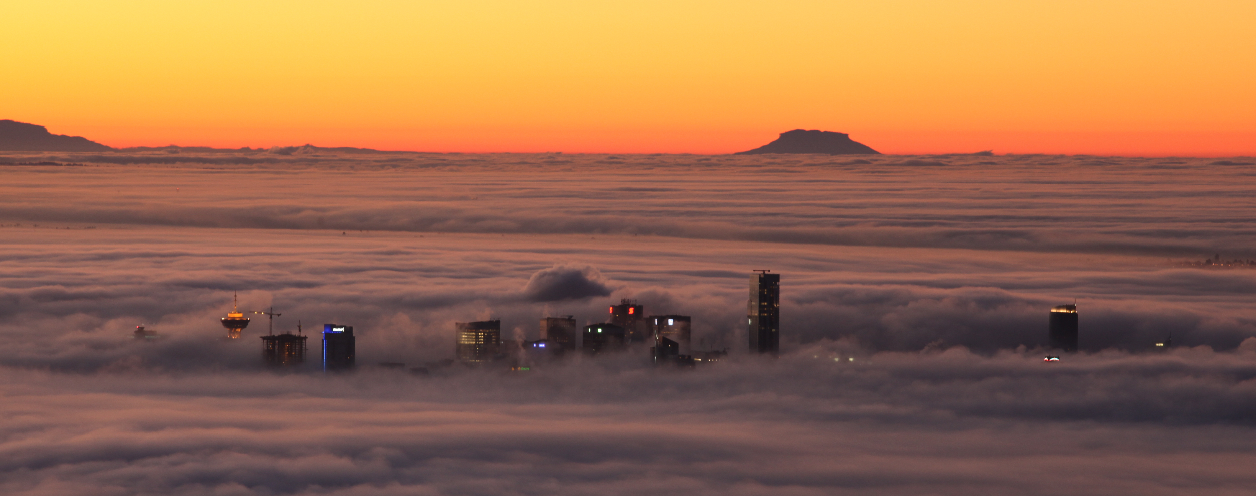
\includegraphics[width=\linewidth]{CypressView}
  \caption{In the Clouds: Vancouver from Cypress Mountain. Note that the teaser may not be wider than the abstract block.}
	\label{fig:teaser}
}

%% Uncomment below to disable the manuscript note
\renewcommand{\manuscriptnotetxt}{}

%% Copyright space is enabled by default as required by guidelines.
%% It is disabled by the 'review' option or via the following command:
% \nocopyrightspace

\vgtcinsertpkg

%%%%%%%%%%%%%%%%%%%%%%%%%%%%%%%%%%%%%%%%%%%%%%%%%%%%%%%%%%%%%%%%
%%%%%%%%%%%%%%%%%%%%%% START OF THE PAPER %%%%%%%%%%%%%%%%%%%%%%
%%%%%%%%%%%%%%%%%%%%%%%%%%%%%%%%%%%%%%%%%%%%%%%%%%%%%%%%%%%%%%%%%

\begin{document}

%% The ``\maketitle'' command must be the first command after the
%% ``\begin{document}'' command. It prepares and prints the title block.

%% the only exception to this rule is the \firstsection command
\firstsection{Introduction}

\maketitle

%% \section{Introduction} %for journal use above \firstsection{..} instead
Safety of students in a university is of utmost importance. The crime rate in an around the university plays a vital role in choosing a school. With this project we intend to help young students and parents make well informed decisions. The motivation behind this visualization is also to help universities to improve security and also to provide students with the required counseling. The Department of Education released this data set which contains the information of campus arrests and crimes in the years 2013, 2014, 2015.\\
The website allows the users to compare universities. However, there is no visualization which portrays the dataset. The problem that this paper addresses is how this dataset can be visualized providing meaningful insight. The dataset has different categories which makes it harder to visualize. The aim of this visualization is to map all the universities which have recorded crimes committed on campus onto the map of the United States of America, and then show the different crime committed in the form histograms.\\
As the dataset is huge and handling such a vast dataset may result in complications while visualizing, we have decided to first make a prototype with all the universities and colleges in the state of Oregon. The next step is to then include all the universities and colleges in the country. The visualization is a good way to represent this data set as it makes it easier for the intended audience to understand the data better. The following sections show the work flow behind the implementation of this visualization.\\

\section{Literary Research and References} \label{research}

The data for crimes committed on campuses in the United States has been required by the Clery Act law to be sent to the government each year.  However, this raw data is of little help to future students and parents as long reports of just numbers are hard to read and hard to find\cite{lipka-2011}.  A web based visualization will enable future students to easily find the crime data without sorting through dense reports.

A study in 2012 showed that students were afraid of crime maps as it made crimes seem more prevalent than they actually were\cite{fuhrmann-huynh-scholz-2013}. For our visualization, the same base numbers are used for each University so each University can be easily compared to one another.  The only downside to this method is that the size of the University is not taken into account which may make smaller Universities disproportionately safer.

Another problem with our data is that it includes some crimes committed off-campus. The problem with this is that locations not on campus can contribute to the crime stats without being actually school related.  A report shows the Casinos near campus can cause spikes in certain crimes.  Robberies and vehicle thefts are increased, but burglaries are lower\cite{Thomas:2011:CRIME}.  However, for our needs this does not change the base crime statistics.

Other problems with our visualization is that it only shows successful crimes that are reported.  Universities have several methods in place to alleviate crime and make their campuses safer\cite{doi:10.1177/0193841X13509815}.  Emergency phones and well lit walkways are just some of the infrastructure in place to counter crime.  In our data, only the resulting crime is reported.

\section{Method and Implementation}

For this visualization, we created a webpage \cite that implements the d3.js v4 package to gather data and present a graphic representation. We had a public dataset \cite with campus crime data from 2013, 2014, and 2015 for colleges all over the united states. From that data, we selected rows pertaining to Oregon colleges (specifically Oregon State University, University of Oregon, and Portland State University) and loaded them as a .csv file into the d3 JavaScript of our webpage. Our visualization creates a dynamic bar chart that changes according to the different filters applied.\\ 
Our group researched several different visualization techniques in the previous section (\nameref{research}) including pie charts, bubble maps, and heap maps that were used to display data. We analyzed the reasoning behind each technique and began to consider what we really want to convey with our visualization. Some visualizations aimed to display proportionalities between geographical areas or data categories. Some visualizations wanted to show concentrations of data for specific regions with heap maps. In our case, we wanted explicit numbers for specific comparisons.\\
Our visualization presents college campus crime date as three main comparisons:
\begin{enumerate}
	\item Liquor, weapon, and drug crimes for the years 2013-2015 for a specific school.
	\item A comparison of each crime type for each year (i.e. weapons crimes of 2013, 2014, and 2015).
	\item And then a comparison of all school's crimes for a given crime type (All Oregon State weapon crimes vs. all University of Oregon weapon crimes vs. all Portland State Weapon Crimes).
\end{enumerate}
\begin{figure}[h]
\label{fig:OverviewDiagram}
\centering
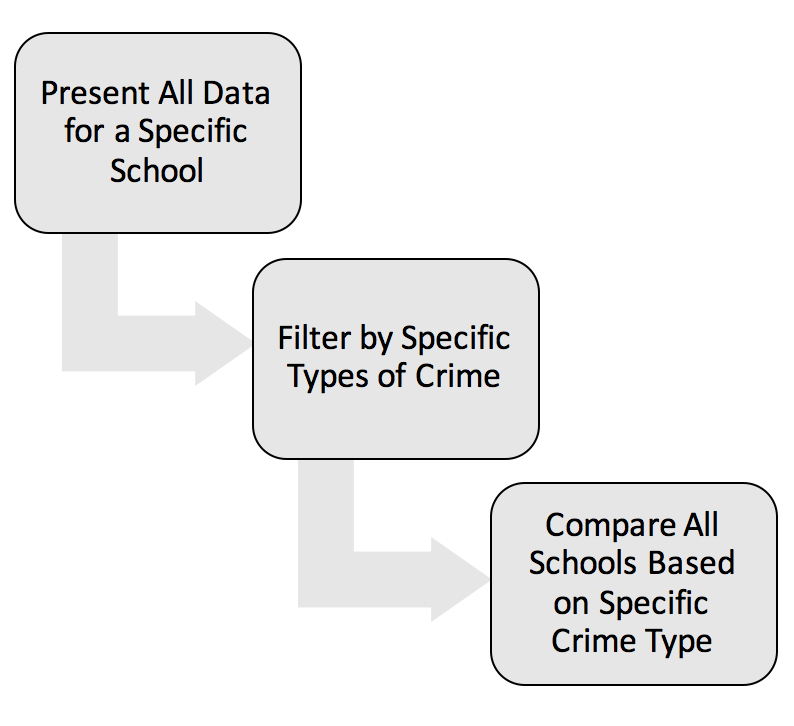
\includegraphics[width=6cm, height=6cm]{method-flow-chart}
\caption{Overview Diagram of Visualization Model}
\end{figure}
We use a simple button group that dynamically changes the d3 svg object according to the desired filter. We accomplish this by updating the dataset given to the d3 axes and bar objects each time a new filter event is activated. 
\subsection{One School, All Data}
Our visualization begins by selecting a school and displaying crime data for weapon crimes, drug crimes, and liquor crimes by year. By clicking on a school node, the webpage calls a JavaScript function buildChart() and passes in a string parameter for the desired college. This function then parses the .csv file and creates arrays for each crime type and year based on college. We used d3.js functions such as nest() and rollup() to combine all data rows for the same college and add the values for each crime category \cite{d3API}.
It then creates a dataset by selecting only data from each array pertaining to the college supplied by the function parameter. Using this dataset, the function appends rectangle objects and axes to the svg element in the HTML of the webpage, and populates each obbject with the corresponding values. This creates a bar graph separated by crime type and year for the specified school. Clicking a different college node on the map will remove all previous rectangles and axes, repopulate the dataset with the corresponding college's data, and rebuild the bar graph. 
\begin{figure}[h]
\label{fig:OneSchoolAllData}
\centering
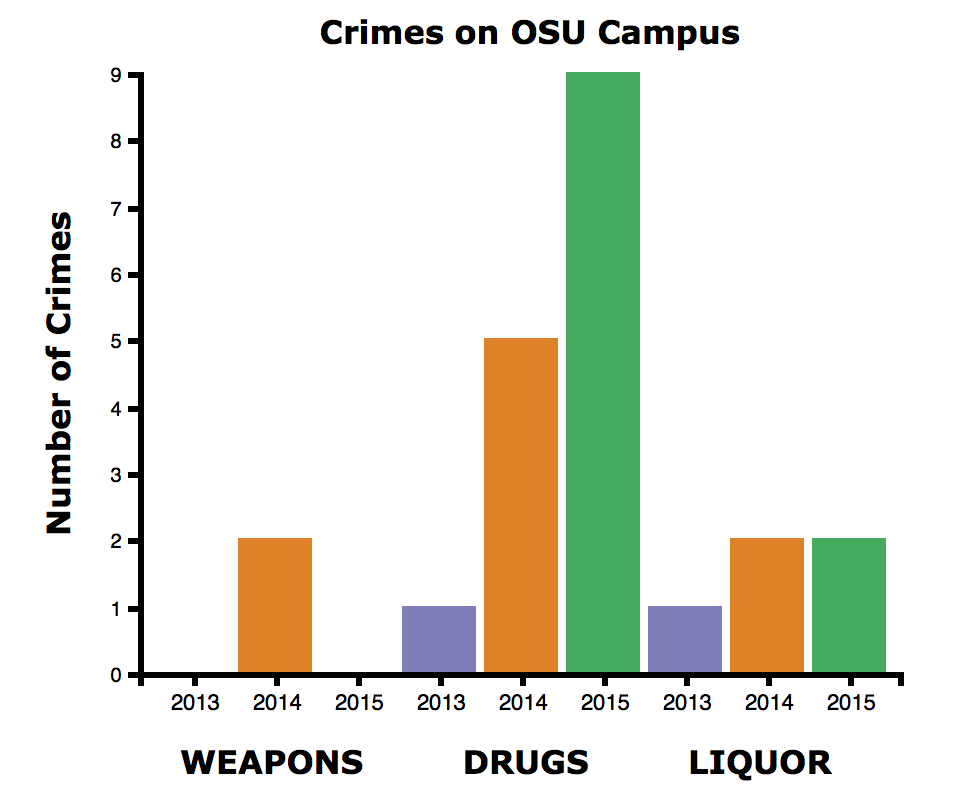
\includegraphics[width=9cm, height=9cm]{OneSchoolAllData}
\caption{A bar graph of all crimes for Oregon State University organized by crime type and year.}
\end{figure}
\section{Conclusion}

Insert Conclusion.


%% if specified like this the section will be committed in review mode
\acknowledgments{
The authors wish to thank A, B, C. This work was supported in part by
a grant from XYZ.}

%\bibliographystyle{abbrv}
\bibliographystyle{abbrv-doi}
%\bibliographystyle{abbrv-doi-narrow}
%\bibliographystyle{abbrv-doi-hyperref}
%\bibliographystyle{abbrv-doi-hyperref-narrow}

\bibliography{crimeoncampus}
\end{document}

